%\documentclass[a4,semhelv,landscape]{seminar}
\documentclass[landscape]{slides}
%\documentclass[pdf, default, slideBW, nocolorBG]{prosper}
\usepackage[left=0.2cm,top=0.2cm,right=0.2cm,bottom=0.2cm,nohead,nofoot]{geometry}
%\def\everyslide{\sffamily}
%\usepackage{fullpage}
\usepackage{graphicx}
\usepackage[usenames]{color}
%\usepackage{color}
\usepackage{verbatim}
\usepackage{nopageno}
\usepackage{setspace}
%\usepackage{times}
% define some nice colors
\definecolor{myred}{rgb}{0.6,0,0}
\definecolor{myblue}{rgb}{0,0.2,0.4}
\definecolor{mygreen}{rgb}{0,0.5,0.0}
\definecolor{mypurple}{cmyk}{0.5,1.0,0.0,0.0}
%\color{myblue}

\begin{document}
%%%%%%%%%%%%%%%%%%%%%%%%%%%%%%%%%%%%%%%%%%%%%%%%%%%%%%%%%%%%%%%%%%%%
%Slide 0 - title
\begin{slide}
\begin{center}
\large{\textbf{Archaeal group I introns}}

\normalsize

Eric Nawrocki

\medskip

\medskip

\small

\begin{tabular}{c}
National Center for Biotechnology Information\\
National Institutes of Health\\
\end{tabular}

\vspace{0.1in}

\includegraphics[width=2.5in]{figs/ncbi-logo}

\end{center}
\end{slide}
%%%%%%%%%%%%%%%%%%%%%%%%%%%%%%%%%%%%%%%%%%%%%%%%%%%%%%%%%%%%%%%%%%%%%%
%%%%%%%%%%%%%%%%%%%%%%%%%%%%%%%%%%%%%%%%%%%%%%%%%%%%%%%%%%%%%%%%%%%%%%%%%%
\begin{slide}
\begin{center}
\textbf{Infernal 1.1 finds 11,000 new group I intron candidates}
\end{center}

%\center{\includegraphics[width=10.5in]{figs/rfam-nar-table1-published-gp1i-yellow}}
\center{\includegraphics[width=10.5in]{figs/rfam-nar-table1-published-gp1i-yellow-top5only}}

\vfill
\end{slide}
%%%%%%%%%%%%%%%%%%%%%%%%%%%%%%%%%%%%%%%%%%%%%%%%%%%%%%%%%%%%%%%%%%%%%%
\begin{slide}
\begin{center}
\textbf{Group I catalytic Introns}
\end{center}
%
\small
\begin{itemize}
\item self splicing ribozymes found in lower eukaryotes, higher
  plants, bacteria and bacteriophages
%\item core secondary structure (modeled by Rfam) consists of 9 paired
%  regions
\item often have ORFs (homing endonucleases) inserted in loop regions
\item genes they are found in:
\begin {itemize}
\item bacteria and mitochondria and chloroplast of lower euks: rRNA, mRNA, and tRNAs
\item higher plants mitochondria and chloroplast: a few tRNA and mRNA genes
\item nuclear lower eukaryotic genomes: only rRNA
%\item Gram positive bacteriophages: widely distributed
%\item Gram negative bacteriophages: T4, T-even and T7-like
\end{itemize}
\end{itemize}

%\center{\includegraphics[height=4in]{figs/gp1-schematic-small.png}}
\center{\includegraphics[height=4.5in]{figs/gp1-schematic-big.png}}


\vfill
\end{slide}
%%%%%%%%%%%%%%%%%%%%%%%%%%%%%%%%%%%%%%%%%%%%%%%%%%%%%%%%%%%%%%%%%%%%%%%%%%
\begin{slide}
\center{\includegraphics[height=8in]{figs/RF00028-ss-info-ss-1}}
\vfill
\end{slide}
%%%%%%%%%%%%%%%%%%%%%%%%%%%%%%%%%%%%%%%%%%%%%%%%%%%%%%%%%%%%%%%%%%%%%%%%%%
\begin{slide}
\center{\includegraphics[height=8in]{figs/RF00028-ss-mutinfo-ss-1}}
\vfill
\end{slide}
%%%%%%%%%%%%%%%%%%%%%%%%%%%%%%%%%%%%%%%%%%%%%%%%%%%%%%%%%%%%%%%%%%%%%%%%%%
\begin{slide}
\begin{center}
\small
\textbf{GISSD\footnote{Y. Zhou et. al, NAR, 2008. 36(suppl
    1), D31-D37.}: Group I Intron Sequence and Structure Database}
\end{center}

\center{\includegraphics[width=10in]{figs/gissd-banner}}

\center{\includegraphics[width=10in]{figs/gissd-alistat-ss-1}}

\vfill
\end{slide}
%%%%%%%%%%%%%%%%%%%%%%%%%%%%%%%%%%%%%%%%%%%%%%%%%%%%%%%%%%%%%%%%%%%%%%%%%%
\begin{slide}
\begin{center}
\textbf{Searching Rfamseq with GISSD models}
\end{center}

%\small
%\begin{center}
%\begin{tabular}{l|r|rrr|r}
%\tt
%        & \# RF00028 & \# hits   & \# hits& \# hits& total     \\
%type    & seed seqs  & total     & common & unique & CPU hours \\ \hline
%IA1     & 3          &  814      & 385    & 425    & 1076 \\
%IA2     & 1          &  1722     & 823    & 899    & 50 \\
%IA3     &            &   958     & 401    & 557    & 14 \\
%IB1     &            &  3949     & 1033   & 2916   & 32 \\
%IB2     &            & 1861     & 467    & 1394   & 31 \\
%IB3     &            & 479     & 136    & 343    & 40 \\
%IB4     &  1         & 5717     & 2400   & 3317   & 39 \\
%IC1     &  3         & 8475     & 5385   & 3090   & 24 \\
%IC2     &            & 4870     & 3858   & 1012   & 22 \\
%IC3     & 4          & 72692     & 66033  & 6659   & 136 \\
%ID      &            & 572     & 0      & 572    & 29 \\
%IE1     &            & 1305     & 10     & 1295   & 12 \\
%IE2     &            & 1377     & 8      & 1369   & 12 \\
%IE3     &            & 1379     & 1      & 1378   & 13 \\
%        &            &          &        &        &    \\
%total   & 12         & 106170*   & 80940* & 25226  & 1530 \\
%        &           &           &        &    \\
%RF00028 & -         & 71421     & 71421  & -      & 125 \\
%\end{tabular}


\small
\begin{center}
\begin{tabular}{l|r|rrr}
\tt
        & \# RF00028 & \# hits   & \# hits& \# hits\\
type    & seed seqs  & total     & common & unique \\ \hline
IA1     & 3          &  814      & 385    & 425    \\
IA2     & 1          &  1722     & 823    & 899    \\
IA3     &            &   958     & 401    & 557    \\
IB1     &            &  3949     & 1033   & 2916   \\
IB2     &            & 1861     & 467    & 1394   \\
IB3     &            & 479     & 136    & 343    \\
IB4     &  1         & 5717     & 2400   & 3317   \\
IC1     &  3         & 8475     & 5385   & 3090   \\
IC2     &            & 4870     & 3858   & 1012   \\
IC3     & 4          & 72692     & 66033  & 6659   \\
ID      &            & 572     & 0      & 572    \\
IE1     &            & 1305     & 10     & 1295   \\
IE2     &            & 1377     & 8      & 1369   \\
IE3     &            & 1379     & 1      & 1378   \\
        &            &          &        &        \\
%total   & 12         & 106170*   & 80940* & 25226*  \\
total   & 12         & 106170*   & 80940* &  16842 \\
        &           &           &        \\
RF00028 & -         & 71421     & 71421  & -      \\
\end{tabular}

\begin{description}
\item[*] contains overlaps
\end{description}


\end{center}

\vfill
\end{slide}
%%%%%%%%%%%%%%%%%%%%%%%%%%%%%%%%%%%%%%%%%%%%%%%%%%%%%%%%%%%%%%%%%%%%%%%%%
\begin{slide}
\center{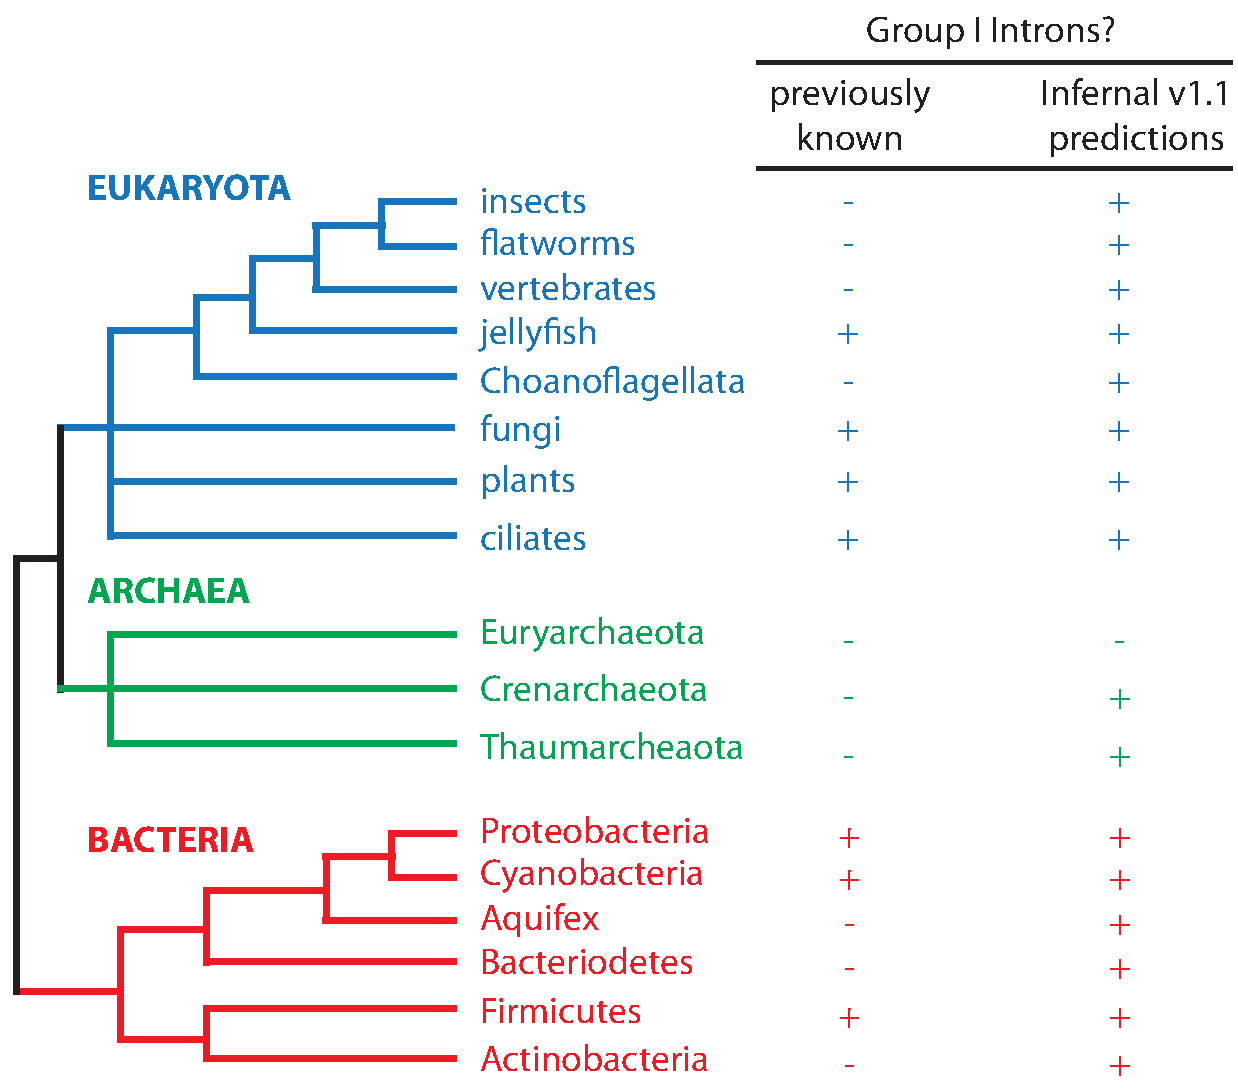
\includegraphics[height=8in]{figs/sean-slide-012215-gp1i-distro}}
\vfill
\end{slide}
%%%%%%%%%%%%%%%%%%%%%%%%%%%%%%%%%%%%%%%%%%%%%%%%%%%%%%%%%%%%%%%%%%%%%%%%%
\begin{slide}
\begin{center}
\textbf{Homology searches for group I introns in Archaea}
\end{center}
%
\small
\begin{itemize}
\item downloaded all archaeal sequences in GenBank (6.7Gb as of Sept
  2017)
\item searched archaeal sequences with all GISSD models + RF00028 with
  default cmsearch parameters and with \texttt{--anytrunc}
\item 95 non-overlapping hits with $E < 0.01$
  corresponding\footnote{as determined via manual sequence analysis by Tom Jones} to 39
  group I intron candidates (12 IA3 and 27 IB4)
\item 30/39 introns have at least one hit with $E < 10^{-10}$ 
\item 36 within LSU rRNA, 3 within SSU rRNA
\item All IA3s are in one of two LSU insertion positions:
  \begin{itemize}
  \item LSU/2593 (N=10)
  \item LSU/2500 (N=2)
  \end{itemize}
\item All IB4s are in one of two LSU insertion positions and one SSU
  position:
  \begin{itemize}
  \item LSU/1931 (N=15)
  \item LSU/1923 (N=9)
  \item SSU/1498 (N=3)
  \end{itemize}  
\end{itemize}  

\vfill
\end{slide}
%%%%%%%%%%%%%%%%%%%%%%%%%%%%%%%%%%%%%%%%%%%%%%%%%%%%%%%%%%%%%%%%%%%%%%%%%%
\begin{slide}
\begin{center}
\textbf{Archaeal group I introns}
\end{center}

\center{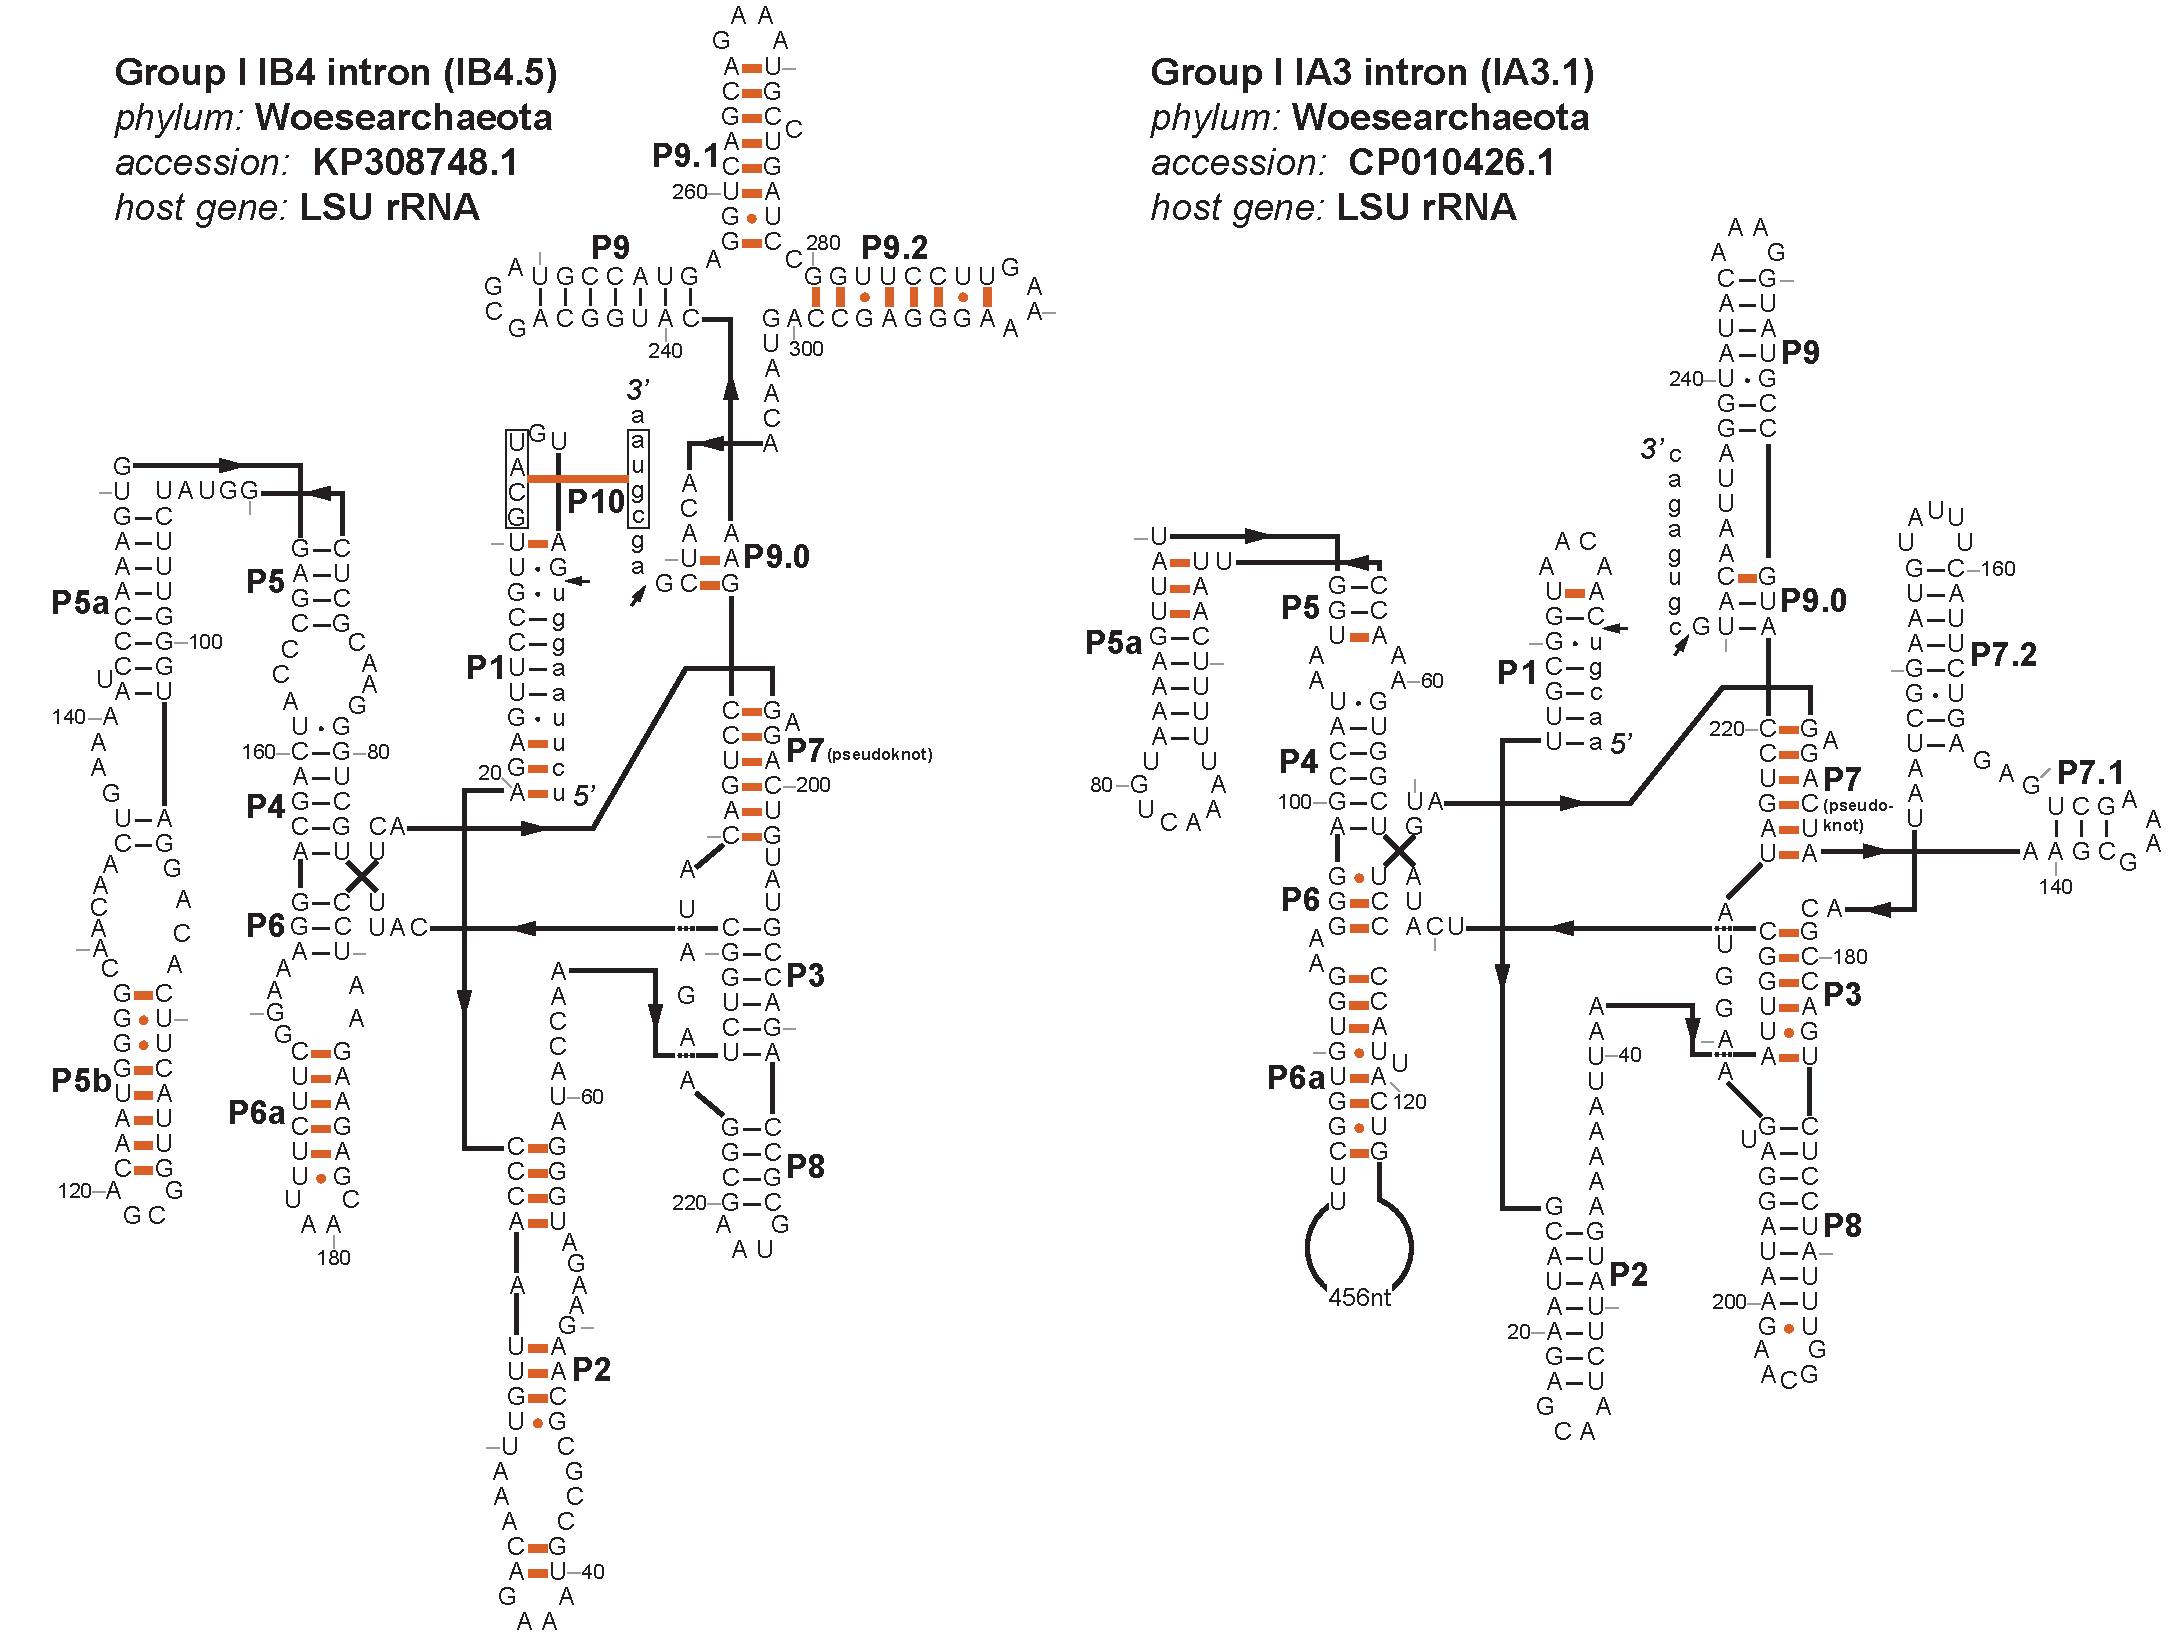
\includegraphics[width=10in]{figs/gp1-fig2-ss}}

\vfill
\end{slide}
%%%%%%%%%%%%%%%%%%%%%%%%%%%%%%%%%%%%%%%%%%%%%%%%%%%%%%%%%%%%%%%%%%%%%%%%%
\begin{slide}
\begin{center}
\textbf{Could archaeal group I introns have evolved into BHB introns?}
\end{center}
\center{\includegraphics[width=8in]{figs/Tocchini-Valentini-title-screenshot}}\footnote{PNAS March 22, 2011. 108 (12) 4782-4787;}

\textbf{Archaeal group I introns can occur in same host gene as BHB introns}

\center{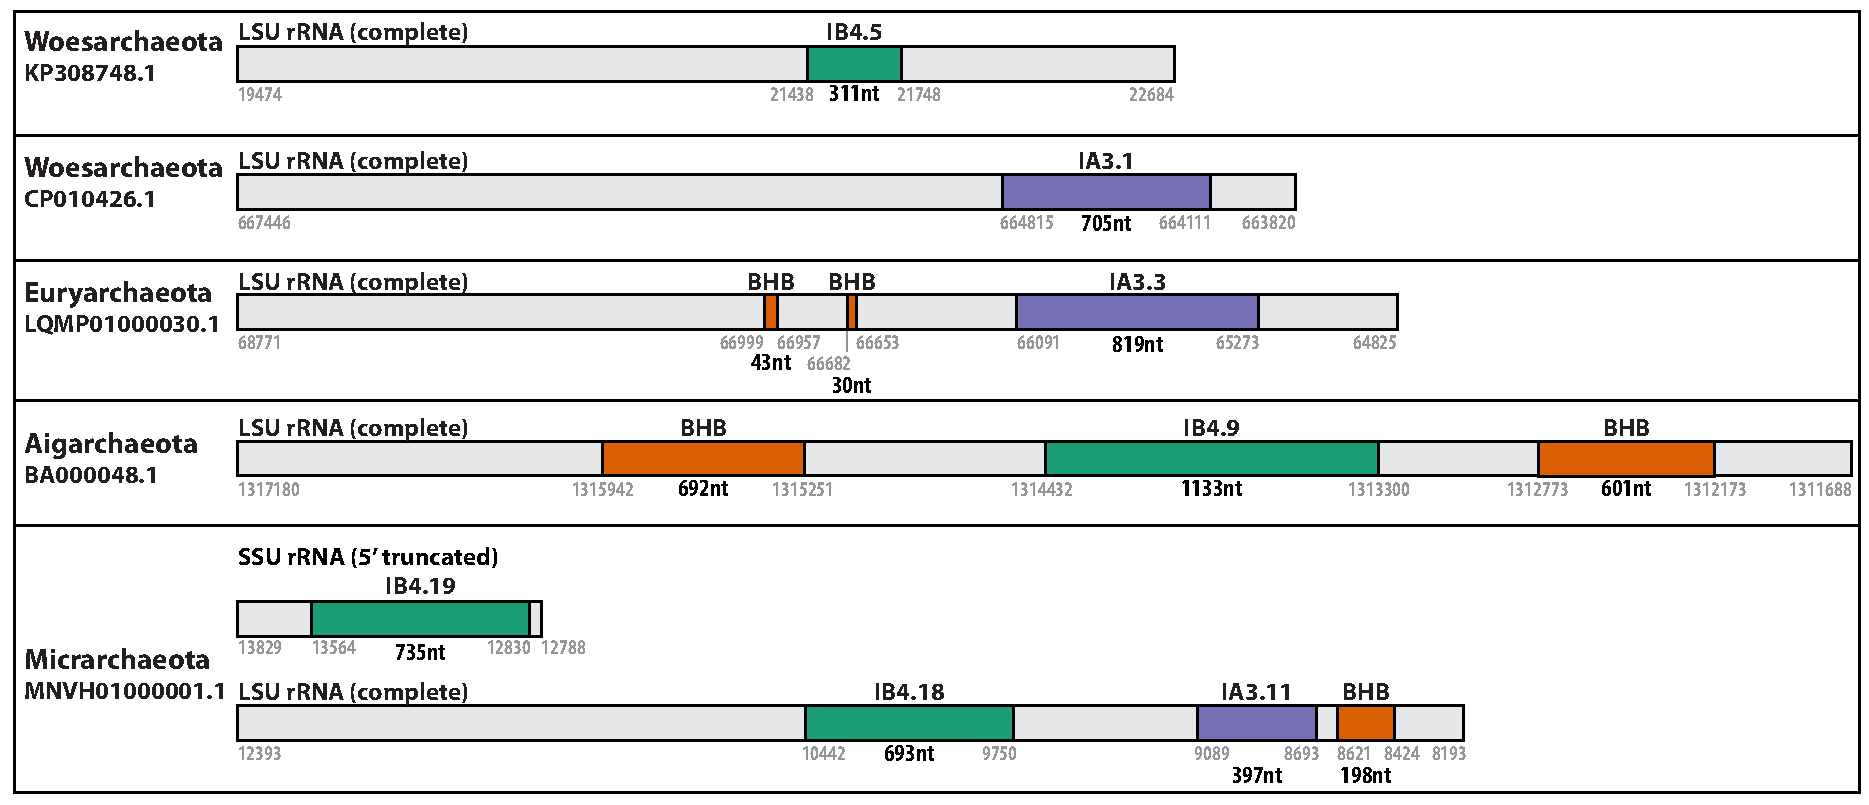
\includegraphics[width=10in]{figs/gp1-fig1-schematic}}
\vfill
\end{slide}
%%%%%%%%%%%%%%%%%%%%%%%%%%%%%%%%%%%%%%%%%%%%%%%%%%%%%%%%%%%%%%%%%%%%%%%%%
\begin{slide}
\begin{center}
\textbf{Group I introns are widespread in Archaea}
\end{center}

\center{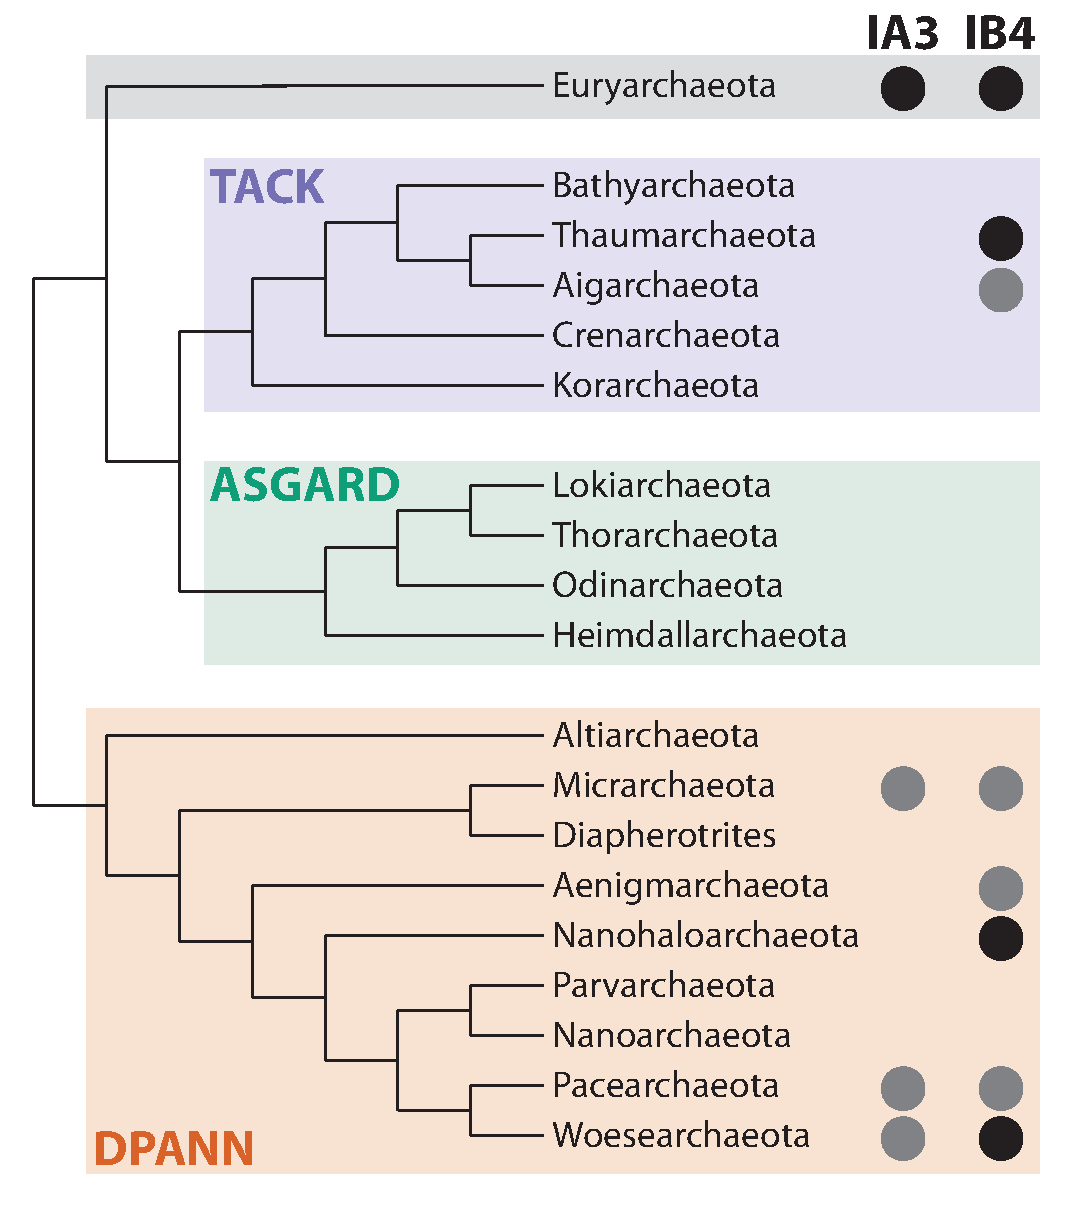
\includegraphics[height=6.5in]{figs/gp1-fig3-cladogram}}

\vfill
\end{slide}
%%%%%%%%%%%%%%%%%%%%%%%%%%%%%%%%%%%%%%%%%%%%%%%%%%%%%%%%%%%%%%%%%%%%%%%%%
\begin{slide}

\large
\begin{center}
\large{\textbf{Acknowledgements}} \\

\normalsize
\vspace{0.5in}

\textbf{Harvard} \\
Sean Eddy \\
Tom Jones \\

\vspace{0.5in}
\textbf{Group I Intron Sequence and Structure Database (GISSD)} \\
Yu Zhou \\
Chen Lu \\
Qi-Jia Wu \\
Yu Wang \\
Zhi-Tao Sun \\
Jia-Cong Deng \\
Yi Zhang \\

\vspace{0.5in}

\textbf{NCBI} \\
Alejandro Sch\"{a}ffer \\
David Landsman \\
Jim Ostell \\
David Lipman \\


\end{center}

\vfill
\end{slide}
%%%%%%%%%%%%%%%%%%%%%%%%%%%%%%%%%%%%%%%%%%%%%%%%%%%%%%%%%%%%%%%%%%%%%%
%%%%%%%%%%%%%%%%%%%%%%%%%%%%%%%%%%%%%%%%%%%%%%%%%%%%%%%%%%%%%%%%%%%%%%
\end{document}
%%%%%%%%%%%%%%%%%%%%%%%%%%%%%%%%%%%%%%%%%%%%%%%%%%%%%%%%%%%%%%%%%%%%%%
%%%%%%%%%%%%%%%%%%%%%%%%%%%%%%%%%%%%%%%%%%%%%%%%%%%%%%%%%%%%%%%
\begin{slide}

\large
\begin{center}
\large{\textbf{Acknowledgements}} \\

\vspace{0.5in}

\normalsize
%\begin{tabular}{llllll}
%Sean Eddy           & & & & & Michael Brent \\ 
%Elena Rivas         & & & & & Jeremy Buhler \\
%Tom Jones           & & & & & Justin Fay \\
%Diana Kolbe         & & & & & Jeff Gordon \\
%Seolkyoung Jung     & & & & & Rob Mitra \\
%Sergi Castellano    & & & & & Gary Stormo \\
%Fred Davis          & & & & & \\
%Lee Henry           & & & & & \\
%Michael Farrar      & & & & & \\
%Travis Wheeler      & & & & & \\
\begin{tabular}{l|l}
\textbf{Harvard/Janelia} & \textbf{EBI (Rfam)} \\ \hline
{\bf Sean Eddy}     & {\bf Alex Bateman} \\
Elena Rivas         & {\bf Rob Finn} \\
Travis Wheeler      & {\bf Sarah Burge} \\ 
{\bf Tom Jones}     & {\bf Evan Floden} \\
Diana Kolbe         & John Tate \\
                    & Jen Daub \\
Rob Finn            & \\
Jody Clements       & \\
Michael Farrar      & \\
\end{tabular}

%\includegraphics[height=3in]{figs/jfrc-banner1}

\end{center}

\vfill
\end{slide}
%%%%%%%%%%%%%%%%%%%%%%%%%%%%%%%%%%%%%%%%%%%%%%%%%%%%%%%%%%%%%%%%%%%%%%
\begin{slide}
\begin{center}
\textbf{Is the added complexity worth it? \\
  RMARK: a challenging \underline{internal} RNA homology search
  benchmark}

\includegraphics[width=10in]{figs/rmark-tree-1}
\end{center}

\vfill
\end{slide}
%%%%%%%%%%%%%%%%%%%%%%%%%%%%%%%%%%%%%%%%%%%%%%%%%%%%%%%%%%%%%%%%%%%%%%
\begin{slide}
\begin{center}
\textbf{Is the added complexity worth it? \\
  RMARK: a challenging \underline{internal} RNA homology search
  benchmark}

\includegraphics[width=10in]{figs/rmark-tree-2}
\end{center}

\vfill
\end{slide}
%%%%%%%%%%%%%%%%%%%%%%%%%%%%%%%%%%%%%%%%%%%%%%%%%%%%%%%%%%%%%%%%%%%%%%
\end{document}
